\ifx\wholebook\relax \else
% ------------------------

\documentclass{article}
\usepackage[en]{../../../prelude}

\setcounter{page}{1}

\begin{document}

%--------------------------

% ================================================================
%                 COVER PAGE
% ================================================================

\title{Radix tree, Trie and Prefix Tree}

\author{Larry~LIU~Xinyu
\thanks{{\bfseries Larry LIU Xinyu } \newline
  Email: liuxinyu95@gmail.com \newline}
  }

\maketitle
\fi

\markboth{Radix tree, Trie and Prefix Tree}{Elementary algorithms}

\ifx\wholebook\relax
\chapter{Radix tree, Trie and Prefix Tree}
\numberwithin{Exercise}{chapter}
\fi

%{\bfseries Corresponding Author:} Larry LIU Xinyu


% ================================================================
%                 Introduction
% ================================================================
\section{Introduction}
\label{introduction}
\index{Radix tree}

The binary trees introduced so far store information in nodes. Edge
can also be used to store information.
Radix trees including Trie and prefix tree are important data structures in
information retrieving and manipulating.
They were found in 1960s. And are widely used in
compiler design\cite{okasaki-int-map}, and bio-information area, such as
DNA pattern matching \cite{wiki-suffix-tree}.

\begin{figure}[htbp]
  \centering
  \includegraphics[scale=0.4]{img/radix-tree.ps}
  \caption{Radix tree.} \label{fig:radix-tree}
\end{figure}

Figure \ref{fig:radix-tree} shows a radix tree(\cite{CLRS} pp. 269).
It contains strings of bit 1011, 10, 011, 100 and 0.
When searching a key $k=(b_0b_1...b_n)_2$, we
take the first bit $b_0$ (MSB from left), check if it is 0 or 1, if it
is 0, we turn left, else turn right for 1. Then we take the second bit and
repeat this search till either meet a leaf node or finish all the $n$ bits.

The radix tree needn't store keys in node at all. The
information is represented by edges. The nodes marked with keys
in the above figure are only for illustration purpose.

Another idea is to represent the key in integer instead of string.
Because integer can be in binary format to save space. The speed
is also fast as we can use bit-wise manipulation in
most programming environments.

% ================================================================
%                 Int Trie
% ================================================================
\section{Integer Trie}
\label{int-trie}
\index{Integer trie}

The data structure shown in figure \ref{fig:radix-tree} is
often called as \emph{binary trie}.
Trie is invented by Edward Fredkin. It comes from ``retrieval'', pronounce
as /'tri:/ by the inventor, while it is pronounced /'trai/ ``try''
by other authors \cite{wiki-trie}. Trie is also called prefix tree.
A binary
trie is a special binary tree in which the placement of each key is controlled by
its bits, each 0 means `go left' and each 1 means `go
right'\cite{okasaki-int-map}.

Because integer can be represented in binary format, we can use it
instead of 0, 1 string. When insert a new integer to the trie, we
change it to binary form, then examine
the first bit, if it is 0, we recursively
insert the rest bits to the left sub-tree; otherwise if it is 1, we insert
into the right sub-tree.

There is a problem when treat the key as integer. Consider a binary
trie shown in figure \ref{fig:big-endian-trie}. If represented in
0, 1 strings, all the three keys are different although they are equal integers.
Where should we insert decimal 3 to this trie?

\begin{figure}[htbp]
  \centering
  \includegraphics[scale=0.4]{img/big-endian-trie.ps}
  \caption{A big-endian trie.} \label{fig:big-endian-trie}
\end{figure}

One approach is to treat all the prefix zero as effective bits.
Suppose the integer is represented with 32-bits, If we want to insert key 1,
it ends up with a tree of 32 levels.
There are 31 nodes, each only has the left sub-tree. the last node only has
the right sub-tree. It is very inefficient in terms of space.

Okasaki shows a method to solve this problem in \cite{okasaki-int-map}. Instead of
using big-endian integer, we can use the little-endian integer to represent key.
Thus decimal integer 1 is represented as binary 1. When insert it to the empty binary
trie, the result is a trie with a root and a right leaf.
There is only 1 level. decimal 2 is represented as 01, and decimal 3 is $(11)_2$
in little-endian binary format. There is no need to add
any prefix 0, the position in the trie is uniquely determined.

%=========================================================================
%       Definition of integer trie
%=========================================================================
\subsection{Definition of integer Trie}
We can use the binary tree structure to define the littel-endian binary trie.
A binary trie node is either empty, or a branch. The branch
node contains a left child, a right node, and optional value as the
satellite data.
The left sub-tree is encoded as 0 and the right sub-tree
is encoded as 1.

The following example Haskell code defines the integer trie as algebraic data type.

\lstset{language=Haskell}
\begin{lstlisting}
data IntTrie a = Empty
               | Branch (IntTrie a) (Maybe a) (IntTrie a)
\end{lstlisting}

The below Python example provides the corresponding imperative definition.

\lstset{language=Python}
\begin{lstlisting}
class IntTrie:
    def __init__(self):
        self.left = self.right = None
        self.value = None
\end{lstlisting}


% ================================================================
%               Insertion of integer trie
% ================================================================
\subsection{Insertion}
\index{Integer trie!insert}

Because the definition of the integer trie is recursive, it's strightforward to define the insertion algorithm recursively.
If the lowest bit is 0, the key to be inserted is even, we recursively insert it
to the left sub-tree; otherwise if the lowest bit is 1, the key is odd,
then the recursive insertion is applied to the right. we next divide the key by 2 to get
rid of the lowest bit. For trie $T$,
denote the left and right sub-trees as $T_l$ and $T_r$ respectively.
Thus $T = (T_l, v', T_r)$, where $v'$ is the optional satellite data.
If $T$ is empty, then $T_l$, $T_r$ and $v'$ are defined as empty as well.

\be
insert(T, k, v) = \left \{
  \begin{array}
  {r@{\quad:\quad}l}
  (T_l, v, T_r) & k = 0 \\
  (insert(T_l, k / 2, v), v', T_r) & even(k) \\
  (T_l, v', insert(T_r, \lfloor k / 2 \rfloor, v)) & otherwise
  \end{array}
\right.
\ee

If the key to be inserted already exists, this algorithm just
overwrites the previous stored data. It can be replaced with
other alternatives, such as to store the data in a linked-list.

Figure \ref{fig:int-trie} shows an example trie. It's generated by inserting the key-value pairs
\{$ 1 \rightarrow a, 4 \rightarrow b, 5 \rightarrow c, 9 \rightarrow d$\} to the empty trie.

\begin{figure}[htbp]
  \centering
  \includegraphics[scale=0.5]{img/int-trie.ps}
  \caption{A little-endian integer binary trie for the map
          \{$ 1 \rightarrow a, 4 \rightarrow b, 5 \rightarrow c, 9 \rightarrow d$\}.}
  \label{fig:int-trie}
\end{figure}

The following Haskell example program implements the insertion
algorithm.

\lstset{language=Haskell}
\begin{lstlisting}
insert t 0 x = Branch (left t) (Just x) (right t)
insert t k x
    | even k = Branch (insert (left t) (k `div` 2) x) (value t) (right t)
    | otherwise = Branch (left t) (value t) (insert (right t) (k `div` 2) x)

left (Branch l _ _) = l
left Empty = Empty

right (Branch _ _ r) = r
right Empty = Empty

value (Branch _ v _) = v
value Empty = Nothing
\end{lstlisting}

We can also define the insertion algorithm imperatively.
As the key is is stored as little-endian integer, when insert a new key,
we extract the bit one by one from the right most.
If it is 0, we go to the left, otherwise for 1, we go to the right.
If the sub-tree is empty, we need create a new node, and repeat this to
the last bit of the key.

%\begin{algorithm}
\begin{algorithmic}[1]
\Function{Insert}{$T, k, v$}
  \If{$T =$ NIL}
    \State $T \gets$ \Call{Empty-Node}{}
  \EndIf
  \State $p \gets T$
  \While{$k \neq 0$}
    \If{\Call{Even?}{$k$}}
      \If{\Call{Left}{$p$} = NIL}
        \State \Call{Left}{$p$} $\gets$ \Call{Empty-Node}{}
      \EndIf
      \State $p \gets$ \Call{Left}{$p$}
    \Else
      \If{\Call{Right}{$p$} = NIL}
        \State \Call{Right}{$p$} $\gets$ \Call{Empty-Node}{}
      \EndIf
      \State $p \gets$ \Call{Right}{$p$}
    \EndIf
    \State $k \gets \lfloor k/2 \rfloor$
  \EndWhile
  \State \Call{Data}{$p$} $\gets v$
  \State \Return $T$
\EndFunction
\end{algorithmic}
%\end{algorithm}

This algorithm takes 3 arguments, a Trie $T$, a key $k$, and the satellite
data $v$. The following example Python program implements the insertion algorithm.
It uses bit-wise operation to test whether a number is even or odd, and shift
the bit to right as division.

\lstset{language=Python}
\begin{lstlisting}
def insert(t, key, value = None):
    if t is None:
        t = IntTrie()
    p = t
    while key != 0:
        if key & 1 == 0:
            if p.left is None:
                p.left = IntTrie()
            p = p.left
        else:
            if p.right is None:
                p.right = IntTrie()
            p = p.right
        key = key >> 1  # key / 2
    p.value = value
    return t
\end{lstlisting}

For a given integer $k$ with $m$ bits in binary, the insertion algorithm
goest into $m$ levels. The performance is bound to $O(m)$ time.

% ================================================================
%               Look up the integer binary trie
% ================================================================
\subsection{Look up}
\index{Integer trie!look up}

To look up key $k$ in the little-endian integer binary trie,
if the trie is empty, the looking up fails; if $k=0$, then we return the data stored
in the current node; if the last bit is 0, we recursively look up the
left sub-tree; otherwise we look up the right sub-tree.

\be
lookup(T, k) =  \left \{
  \begin{array}
  {r@{\quad:\quad}l}
  \phi & T = \phi \\
  d & k = 0 \\
  lookup(T_l, k / 2) & even(k) \\
  lookup(T_r, \lfloor k / 2 \rfloor) & otherwise
  \end{array}
\right.
\ee

The following Haskell example program implements the recursive
look up algorithm.

\lstset{language=Haskell}
\begin{lstlisting}
search Empty k = Nothing
search t 0 = value t
search t k = if even k then search (left t) (k `div` 2)
             else search (right t) (k `div` 2)
\end{lstlisting}

The look up algorithm can also be realized imperatively. We examine each
bit of $k$ from the lowest one. We go left if the bit is 0, otherwise,
go right. The looking up completes when all bits are consumed.

\begin{algorithmic}[1]
\Function{Lookup}{$T, k$}
  \While{$k \neq 0 \land T \neq $NIL}
    \If{ \Call{Even?}{$k$} }
      \State $T \gets$ \Call{Left}{$T$}
    \Else
      \State $T \gets$ \Call{Right}{$T$}
    \EndIf
    \State $k \gets \lfloor k/2 \rfloor$
  \EndWhile
  \If{$T \neq $ NIL}
    \State \Return \Call{Data}{$T$}
  \Else
    \State \Return not found \EndIf
\EndFunction
\end{algorithmic}

Below example Python program implements the looking up algorithm.

\lstset{language=Python}
\begin{lstlisting}
def lookup(t, key):
    while t is not None and k != 0:
        if key & 1 == 0:
            t = t.left
        else:
            t = t.right
        key = key >> 1
    return None if t is None else t.value
\end{lstlisting}

The looking up algorithm is bound to $O(m)$ time, where $m$ is the
number of bits of the key.

% ================================================================
%               Int Tree (Patricia, int prefix tree)
% ================================================================
\section{Integer prefix tree}
\label{int-patricia}
\index{Integer Patricia}
\index{Integer prefix tree}

Trie has some drawbacks. It occupies a lot of
spaces. As shown in figure \ref{fig:int-trie}, the real data is mostly stored in leafs.
It's very common that an integer binary trie contains many nodes only have one child.
One idea is to compress the chained nodes to one.
Integer prefix tree is such a data structure invented by
Donald R. Morrison in 1968, who named it as 'Patricia'. It stands for \textbf{P}ractical \textbf{A}lgorithm \textbf{T}o \textbf{R}etrieve \textbf{I}nformation \textbf{C}oded \textbf{I}n \textbf{A}lphanumeric\cite{patricia-morrison}. It is another kind of prefix tree. We call it integer tree in this book.

Okasaki provided the implementation of integer tree in \cite{okasaki-int-map}.
If merge the chained nodes which have only one child together in figure \ref{fig:int-trie}, we can get a integer tree as shown in figure \ref{fig:little-endian-patricia}.

\begin{figure}[htbp]
  \centering
  \includegraphics[scale=0.5]{img/little-endian-patricia.ps}
  \caption{Little endian integer tree for the map
     \{$ 1 \rightarrow a, 4 \rightarrow b, 5 \rightarrow c, 9 \rightarrow d$\}.}
  \label{fig:little-endian-patricia}
\end{figure}

From this figure, we can find the key of the branch node is the
longest common prefix for its descendant trees.
They branches out at certain bit. Integer tree saves a lot of space compare
to trie.

Different from integer trie, padding bits of zero don't cause issue
with the big endian integer tree. All zero bits before MSB are omitted to
save the space. Okasaki list some significant advantages of big endian
integer tree in \cite{okasaki-int-map}.

% ================================================================
%                 Definition of int tree
% ================================================================
\subsection{Definition}

Integer prefix tree is a special binary tree. It is either
empty or a node. There are two different types of node:

\begin{itemize}
\item A leaf contains integer key and optional satellite data;
\item Or a branch node with the left and right sub-trees. The
two children share the \textbf{longest common prefix} bits for their keys.
For the left child, the next bit in the key is zero, while it's one
for the right child.
\end{itemize}

The following Haskell example code defines integer tree accordingly.

\lstset{language=Haskell}
\begin{lstlisting}
type Key = Int
type Prefix = Int
type Mask = Int

data IntTree a = Empty
               | Leaf Key a
               | Branch Prefix Mask (IntTree a) (IntTree a)
\end{lstlisting}

In the branch node, we use a mask number to tell from which bit the sub-trees differ.
The mask is power of 2, which is $2^n$ for some non-negative integer $n$, all
bits that are lower than $n$ don't belong to the common prefix.

The following example Python code defines integer tree with auxiliary functions.

\lstset{language=Python}
\begin{lstlisting}
class IntTree:
    def __init__(self, key = 0, value = None):
        self.key = key
        self.value = value
        self.prefix = key
        self.mask = 1
        self.left = self.right = None

    def isleaf(self):
        return self.left is None and self.right is None

    def replace(self, x, y):
        if self.left == x:
            self.left = y
        else:
            self.right = y

    def match(self, k):
        return maskbit(k, self.mask) == self.prefix
\end{lstlisting}

Where match tests if the prefix stored in the node are same as the given key
before the mask bit. It's explained in the next section.

% ================================================================
%                 Insertion of int tree
% ================================================================
\subsection{Insertion}
\index{Integer tree!insert}
When insert a key, if the tree is empty, we create a leaf node as shown in figure
\ref{fig:int-patricia-insert-a}.

\begin{figure}[htbp]
  \centering
    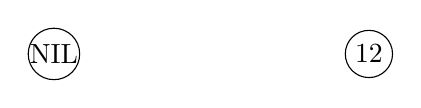
\begin{tikzpicture}[scale=1,
      treenode/.style={circle, draw, inner sep= 0pt, minimum size = .6cm}]
    \node[treenode] at (-2, 0) {NIL};
    \node[treenode] at (2, 0) {12};
    \end{tikzpicture}
  %\includegraphics[scale=1]{img/int-patricia-insert-a.ps}
  \caption{Left: the empty tree; Right: After insert key 12.}
  \label{fig:int-patricia-insert-a}
\end{figure}

If the tree is a singleton leaf node $x$, we create a new leaf $y$,
put the key and the value into it. After that, we need create a new branch
node, set $x$ and $y$ as the two sub-trees.
In order to determine if $y$ should be on the left or right, we need
find the longest common prefix of $x$ and $y$. For example if $key(x)$
is 12 ($(1100)_2$ in binary), $key(y)$ is 15 ($(1111)_2$ in binary), then the longest
common prefix is $(11oo)_2$. Where $o$ denotes the bits we don't care about.
We can use another integer to mask those bits.
In this case, the mask number is 4 (100 in binary).
The next bit after the longest common prefix presents $2^1$. This bit is
0 in $key(x)$, while it is 1 in $key(y)$. We should set $x$ as the left
sub-tree and $y$ as the right sub-tree. Figure \ref{fig:int-patricia-insert-b}
shows this example.

\begin{figure}[htbp]
  \centering
  \includegraphics[scale=0.7]{img/int-patricia-insert-b.ps}
  \caption{Left: A tree with a singleton leaf 12; Right: After insert key 15.}
  \label{fig:int-patricia-insert-b}
\end{figure}

In case the tree is neither empty, nor a singleton leaf, we need
firstly check if the key to be inserted matches the longest common
prefix recorded in the root.
Then recursively insert the key to the left or right
according to the next bit of the longest common prefix.
For example, if insert key 14 ($(1110)_2$ in binary) to the result tree
in figure \ref{fig:int-patricia-insert-b}, since the common prefix is
$(11oo)_2$, and the next bit (the bit of $2^1$) is 1, we need recursively
insert to the right sub-tree.

If the key to be inserted doesn't match the longest
common prefix in the root, we need branch a new leaf
out. Figure \ref{fig:int-patricia-insert-c} shows these two different cases.

\begin{figure}[htbp]
  \centering
  \subfloat[Insert key 14. It matches the longest common prefix $(1100)_2$; 14 is then recursively inserted to the right sub-tree.]{\includegraphics[scale=0.5]{img/int-patricia-insert-c.ps}}\\
  \subfloat[Insert key 5. It doesn't match the longest common prefix $(1100)_2$, a new leaf is branched out.]{\includegraphics[scale=0.5]{img/int-patricia-insert-d.ps}}
  \caption{Insert key to the branch node.}
  \label{fig:int-patricia-insert-c}
\end{figure}

For a given key $k$ and value $v$, denote $(k, v)$ as the leaf node. For branch
node, denote it in form of $(p, m, T_l, T_r)$, where $p$ is the longest common
prefix, $m$ is the mask, $T_l$ and $T_r$ are the left and right sub-trees.
Summarize the above cases, the insertion algorithm can be defined as below.

\be
insert(T, k, v) = \left \{
  \begin{array}
  {r@{\quad:\quad}l}
  (k, v) & T = \phi \lor T = (k, v') \\
  join(k, (k, v), k', T) & T = (k', v') \\
  (p, m, insert(T_l, k, v), T_r) & T = (p, m, T_l, T_r), match(k, p, m), zero(k, m) \\
  (p, m, T_l, insert(T_r, k, v)) & T = (p, m, T_l, T_r), match(k, p, m), \lnot zero(k, m) \\
  join(k, (k, v), p, T) & T = (p, m, T_l, T_r), \lnot match(k, p, m)
  \end{array}
\right.
\ee

The first clause deals with the edge cases, if $T$ is empty, the result is a leaf
node. If $T$ is a leaf node with the same key, we overwrite the previous
value.

The second clause handles the case that $T$ is a leaf node, but with different
key. Here we branch out another leaf, then extract the longest
common prefix, and determine which leaf should be set as the left sub-tree.
Function $join(k_1, T_1, k_2, T_2)$ does this work. We'll define it later.

The third clause deals with the case that $T$ is a branch node, the
longest common prefix matches the key to be inserted, and the next
bit to the common prefix is zero. Here we need recursively insert
to the left sub-tree.

The fourth clause handles the similar case as the third one, except
that the next bit to the common prefix is one, but not zero. We need
recursively insert to the right sub-tree.

The last clause is for the case that the key to be inserted doesn't
match the longest common prefix in the branch. We need branch
out a new leaf by calling the $join$ function.

We need define function $match(k, p, m)$ to test if the key $k$, has
the same prefix $p$ above the masked bits $m$.
For example, suppose the prefix stored in a branch node is
$(p_np_{n-1} ... p_i...p_0)_2$ in binary, key $k$ is
$(k_nk_{n-1} ... k_i ... k_0)_2$ in binary, and the mask is
$(100...0)_2=2^i$. They match if and only if $p_j=k_j$ for all $j$, that $i \leq j \leq n$.

One solution to realize match is to test if $mask(k, m) = p$ is satisfied.
Where $mask(x, m) = \overline{m-1} \& x$, that we perform bitwise-not of $m-1$, then
perform bitwise-and with $x$.

Function $zero(k, m)$ test the next bit of the common prefix is zero.
With the help of the mask $m$, we can shift $m$ one bit to the right,
then perform bitwise-and with the key.

\be
zero(k, m) = x \& shift_r(m, 1)
\ee

If the mask $m = (100..0)_2 = 2^i$, $k = (k_nk_{n-1}...k_i1...k_0)_2$,
because the bit next to $k_i$ is 1, $zero(k, m)$ returns false value;
if $k = (k_nk_{n-1}...k_i0...k_0)_2$, then the result is true.

Function $join(p_1, T_1, p_2, T_2)$ takes two different prefixes and trees.
It extracts the longest common prefix of $p_1$ and $p_2$, create a
new branch node, and set $T_1$ and $T_2$ as the two sub-trees.

\be
join(p_1, T_1, p_2, T_2) = \left \{
  \begin{array}
  {r@{\quad:\quad}l}
  (p, m, T_1, T_2) & zero(p1, m), (p, m) = LCP(p_1, p_2) \\
  (p, m, T_2, T_1) & \lnot zero(p1, m)
  \end{array}
\right.
\ee

In order to calculate the longest common prefix of $p_1$ and $p_2$,
we can firstly compute bitwise exclusive-or for them, then count
the number of bits in this result, and generate a mask $m = 2^{|xor(p_1,p_2)|}$.
The longest common prefix $p$ can be given by masking the bits with $m$
for either $p_1$ or $p_2$.

\be
p = mask(p_1, m)
\ee

The following Haskell example program implements the insertion algorithm.

\lstset{language=Haskell}
\begin{lstlisting}
import Data.Bits

insert t k x
   = case t of
       Empty -> Leaf k x
       Leaf k' x' -> if k==k' then Leaf k x
                     else join k (Leaf k x) k' t -- t@(Leaf k' x')
       Branch p m l r
          | match k p m -> if zero k m
                           then Branch p m (insert l k x) r
                           else Branch p m l (insert r k x)
          | otherwise -> join k (Leaf k x) p t -- t@(Branch p m l r)

join p1 t1 p2 t2 = if zero p1 m then Branch p m t1 t2
                                else Branch p m t2 t1
    where
      (p, m) = lcp p1 p2

lcp :: Prefix -> Prefix -> (Prefix, Mask)
lcp p1 p2 = (p, m) where
    m = bit (highestBit (p1 `xor` p2))
    p = mask p1 m

highestBit x = if x == 0 then 0 else 1 + highestBit (shiftR x 1)

mask x m = (x .&. complement (m-1)) -- complement means bit-wise not.

zero x m = x .&. (shiftR m 1) == 0

match k p m = (mask k m) == p
\end{lstlisting}

The insertion algorithm can also be realized imperatively.

\begin{algorithmic}[1]
\Function{Insert}{$T, k, v$}
  \If{$T = $ NIL}
    \State $T \gets$ \Call{Create-Leaf}{$k, v$}
    \State \Return $T$
  \EndIf
  \State $y \gets T$
  \State $p \gets$ NIL
  \While{$y$ is not leaf, and \textproc{Match}($k$, \Call{Prefix}{$y$}, \Call{Mask}{$y$})}
    \State $p \gets y$
    \If{\textproc{Zero?}($k$, \Call{Mask}{$y$})}
      \State $y \gets$ \Call{Left}{$y$}
    \Else
      \State $y \gets$ \Call{Right}{$y$}
    \EndIf
  \EndWhile
  \If{$y$ is leaf, and $k = $ \Call{Key}{$y$}}
    \State \Call{Data}{$y$} $\gets v$
  \Else
    \State $z \gets$ \textproc{Branch}($y$, \Call{Create-Leaf}{$k, v$})
    \If{$p = $ NIL}
      \State $T \gets z$
    \Else
      \If{\Call{Left}{$p$} $ = y$}
        \State \Call{Left}{$p$} $\gets z$
      \Else
        \State \Call{Right}{$p$} $\gets z$
      \EndIf
    \EndIf
  \EndIf
  \State \Return $T$
\EndFunction
\end{algorithmic}

Function \textproc{Branch}($T_1, T_2$) does the similar job as what $join$ is defined.
It creates a new branch node, extracts the longest common prefix, sets $T_1$ and
$T_2$ as the two sub-trees.

\begin{algorithmic}[1]
\Function{Branch}{$T_1, T_2$}
  \State $T \gets$ \Call{Empty-Node}{}
  \State $($ \Call{Prefix}{$T$}, \Call{Mask}{$T$} $) \gets$ \textproc{LCP}(\Call{Prefix}{$T_1$}, \Call{Prefix}{$T_2$})
  \If{\textproc{Zero?}(\Call{Prefix}{$T_1$}, \Call{Mask}{$T$})}
    \State \Call{Left}{$T$} $\gets T_1$
    \State \Call{Right}{$T$} $\gets T_2$
  \Else
    \State \Call{Left}{$T$} $\gets T_2$
    \State \Call{Right}{$T$} $\gets T_1$
  \EndIf
  \State \Return $T$
\EndFunction
\end{algorithmic}


The following Python example program implements the insertion algorithm.

\lstset{language=Python}
\begin{lstlisting}
def insert(t, key, value):
    if t is None:
        return IntTree(key, value)
    node = t
    parent = None
    while (not node.isleaf()) and node.match(key):
        parent = node
        if zero(key, node.mask):
            node = node.left
        else:
            node = node.right
    if node.isleaf() and key == node.key:
        node.value = value
    else:
        p = branch(node, IntTree(key, value))
        if parent is None:
            return p
        parent.replace(node, p)
    return t
\end{lstlisting}

The auxiliary functions, \texttt{branch}, \texttt{lcp} etc. are given as below.

\begin{lstlisting}
def maskbit(x, mask):
    return x & (~(mask - 1))

def zero(x, mask):
    return x & (mask >> 1) == 0

def lcp(p1, p2):
    diff = p1 ^ p2
    mask = 1
    while diff != 0:
        diff >>= 1
        mask <<= 1
    return (maskbit(p1, mask), mask)

def branch(t1, t2):
    t = IntTree()
    (t.prefix, t.mask) = lcp(t1.prefix, t2.prefix)
    if zero(t1.prefix, t.mask):
        t.left, t.right = t1, t2
    else:
        t.left, t.right = t2, t1
    return t
\end{lstlisting}

Figure \ref{fig:int-patricia-haskell-insert} shows the example integer tree created
with the insertion algorithm.

\begin{figure}[htbp]
  \centering
  \includegraphics[scale=0.6]{img/int-patricia-haskell-insert.ps}
  \caption{Insert map $1 \rightarrow x, 4 \rightarrow y, 5 \rightarrow z$ into the big-endian integer prefix tree.}
  \label{fig:int-patricia-haskell-insert}
\end{figure}


% ================================================================
%                 Lookup in int patricia tree
% ================================================================
\subsection{Look up}
\index{Integer tree!look up}

If the integer tree $T$ is empty, or it's a singleton leaf with
the key that is different from what we are looking up, the result is empty.
else if the key in the leaf equals, we are done.
If $T$ is a branch node, we need check if the common
prefix matches the subject key, and recursively look up
the sub-tree according to the next bit. If the common prefix doesn't
match the key, then the lookup fails.

\be
lookup(T, k) = \left \{
  \begin{array}
  {r@{\quad:\quad}l}
  \phi & T = \phi \lor (T = (k', v), k' \neq k) \\
  v & T = (k', v), k' = k \\
  lookup(T_l, k) & T = (p, m, T_l, T_r), match(k, p, m), zero(k, m) \\
  lookup(T_r, k) & T = (p, m, T_l, T_r), match(k, p, m), \lnot zero(k, m) \\
  \phi & otherwise
  \end{array}
\right.
\ee

The following Haskell example program implements this recursive
lookup up algorithm.

\lstset{language=Haskell}
\begin{lstlisting}
search t k
  = case t of
      Empty -> Nothing
      Leaf k' x -> if k == k' then Just x else Nothing
      Branch p m l r
             | match k p m -> if zero k m then search l k
                              else search r k
             | otherwise -> Nothing
\end{lstlisting}

The look up algorithm can also be realized imperatively.
Consider the property of integer prefix tree. When look up a
key, if it has common prefix with the root,
then we check the next bit. If
this bit is zero, we then recursively look up the left sub-tree;
otherwise we look up the right sub-tree if the bit is one.

When arrive at the leaf node, we check if the key of the
leaf equals to the one we are looking up.

\begin{algorithmic}[1]
\Function{Look-Up}{$T, k$}
  \If{$T =$ NIL}
    \State \Return $NIL$ \Comment{Not found}
  \EndIf
  \While{$T$ is not leaf, and \textproc{Match}($k$, \Call{Prefix}{$T$}, \Call{Mask}{$T$})}
    \If{\textproc{Zero?}($k$, \Call{Mask}{$T$})}
      \State $T \gets$ \Call{Left}{$T$}
    \Else
      \State $T \gets$ \Call{Right}{$T$}
    \EndIf
  \EndWhile
  \If{$T$ is leaf, and \Call{Key}{$T$} $=k$}
    \State \Return \Call{Data}{$T$}
  \Else
    \State \Return $NIL$ \Comment{Not found}
  \EndIf
\EndFunction
\end{algorithmic}

Below Python example program implements the looking up algorithm.

\lstset{language=Python}
\begin{lstlisting}
def lookup(t, key):
    while t is not None and (not t.isleaf()) and t.match(key):
        if zero(key, t.mask):
            t = t.left
        else:
            t = t.right
    if t is not None and t.isleaf() and t.key == key:
        return t.value
    return None
\end{lstlisting}


% ================================================================
%                 Alphabetic trie
% ================================================================
\section{Alphabetic Trie}
\index{Trie}
Integer based trie and tree can be a good start point. The
Glasgow Haskell Compiler (GHC) utilized the similar integer tree
implementation for several years before 1998\cite{okasaki-int-map}.

If we extend the key from integer to alphabetic
value, Trie and integer tree can be very powerful in solving
textual manipulation problems.

% ================================================================
%                 Definition of Alphabetic trie
% ================================================================
\subsection{Definition}
It's not enough to just use the left and right sub-trees to represent
alphabetic keys. Taking English for example, there are 26 letters.
If we don't care about the case, one solution is to limit the number
of branches (children) to 26. Some simplified implementation defines
the trie with the array of 26 letters.
This can be illustrated as in Figure \ref{fig:trie-of-26}.

\begin{figure}[htbp]
  \centering
  \includegraphics[scale=0.5]{img/trie-of-26.ps}
  \caption{A trie with 26 branches, containing key 'a', 'an', 'another', 'bool',
    'boy' and 'zoo'.}
  \label{fig:trie-of-26}
\end{figure}

Not all the 26 branches contain data. For instance, in Figure \ref{fig:trie-of-26},
the root only has three non-empty branches representing letter 'a',
'b', and 'z'. Other branches such as for letter 'c', are all
empty. We will not show empty branch in the future.

When dealing with case sensitive problems, or handling languages other than English,
there can be more letters. We can use the collection data structures, like Hash map
to define the trie.

Alphabetic trie is either empty or a node. There are two types of node.

\begin{itemize}
\item A leaf node does not have any sub-trees;
\item A branch node contains multiple sub-trees. Each sub-tree is bound to a character.
\end{itemize}

Both leaf and branch can contain optional satellite data. The following Haskell
code shows the example definition.

\lstset{language=Haskell}
\begin{lstlisting}
data Trie a = Trie { value :: Maybe a
                   , children :: [(Char, Trie a)]}

empty = Trie Nothing []
\end{lstlisting}

Below ANSI C example code defines the alphabetic trie. For illustration purpose,
it limits the character set to lower case English letters, from 'a' to 'z'.

\lstset{language=C}
\begin{lstlisting}
struct Trie {
  struct Trie* children[26];
  void* data;
};
\end{lstlisting}


% ================================================================
%                 Insertion of Alphabetic trie
% ================================================================
\subsection{Insertion}
\index{Trie!insert}

When insert to the trie, denote the
key to be inserted as $K = k_1k_2...k_n$, where $k_i$ is the $i$-th
character. $K'$ is the rest of characters except $k_1$, $v'$ is the
data to be inserted.
The trie is in form $T = (v, C)$, where $v$ is the
data store in the trie, $C = \{(c_1, T_1), (c_2, T_2), ..., (c_m, T_m)\}$ is the
collection of sub-trees. It associates a character $c_i$ and the corresponding
sub-tree $T_i$. $C$ is empty for leaf node.

\be
insert(T, K, v') = \left \{
  \begin{array}
  {r@{\quad:\quad}l}
  (v', C) & K = \phi \\
  (v, ins(C, k_1, K', v')) & otherwise.
  \end{array}
\right.
\ee

If the key is empty, the previous value $v$ is overwritten with
$v'$. Otherwise, we need check the children and perform
recursive insertion. This is realized in function $ins(C, k_1, K', v')$.
It examines the (character, sub-tree) pairs in $C$ one by one. Let $C'$ be
the rest of pairs except for the first one. This function
can be defined as below.

\be
ins(C, k_1, K', v') = \left \{
  \begin{array}
  {r@{\quad:\quad}l}
  \{(k_1, insert((\phi, \phi), K', v'))\} & C = \phi \\
  \{k_1, insert(T_1, K', v')\} \cup C' & k_1 = c_1 \\
  \{(c_1, T_1)\} \cup ins(C', k_1, K', v') & otherwise
  \end{array}
\right.
\ee

If $C$ is empty, we create a pair, mapping from character $k_1$ to
a new empty tree (it is not $\phi$, but a node with empty value and empty sub-tree list), and recursively insert the rest characters.
Otherwise, the algorithm locates the child which is mapped
from $k_1$ for further insertion.

The following Haskell example program implements the insertion
algorithm.

\lstset{language=Haskell}
\begin{lstlisting}
insert t []     x = Trie (Just x)  (children t)
insert t (k:ks) x = Trie (value t) (ins (children t) k ks x) where
    ins [] k ks x = [(k, (insert empty ks x))]
    ins (p:ps) k ks x = if fst p == k
                        then (k, insert (snd p) ks x):ps
                        else p:(ins ps k ks x)
\end{lstlisting}

To realize the insertion imperatively, starting from the root, we pick the character
one by one from the string. For each character, we examine which child sub-tree
represents that character. If the corresponding child is empty, a new node is
created. After that, we pick the next character and repeat this process.

After consuming all the characters, we then store the
value bound the key in the node we arrived.

\begin{algorithmic}[1]
\Function{Insert}{$T, k, v$}
  \If{$T = $ NIL}
    \State $T \gets $ \Call{Empty-Node}{}
  \EndIf
  \State $p \gets T$
  \For{each $c$ in $k$}
    \If{\Call{Children}{$p$}[c] = NIL}
      \State \Call{Children}{$p$}[c] $\gets$ \Call{Empty-Node}{}
    \EndIf
    \State $p \gets $ \Call{Children}{$p$}[c]
  \EndFor
  \State \Call{Data}{$p$} $\gets v$
  \State \Return $T$
\EndFunction
\end{algorithmic}

The following example ANSI C program implements the insertion algorithm.

\lstset{language=C}
\begin{lstlisting}
struct Trie* insert(struct Trie* t, const char* key, void* value) {
    int c;
    struct Trie *p;
    if(!t)
        t = create_node();
    for (p = t; *key; ++key, p = p->children[c]) {
        c = *key - 'a';
        if (!p->children[c])
            p->children[c] = create_node();
    }
    p->data = value;
    return t;
}
\end{lstlisting}

Where function \texttt{create\_node} creates new empty node, with all
children initialized to empty.

\begin{lstlisting}
struct Trie* create_node() {
    struct Trie* t = (struct Trie*) malloc(sizeof(struct Trie));
    int i;
    for (i = 0; i < 26; ++i)
        t->children[i] = NULL;
    t->data = NULL;
    return t;
}
\end{lstlisting}

% ================================================================
%                 Look up in Alphabetic trie
% ================================================================
\subsection{Look up}
\index{Trie!look up}

When looking up a key, we start from the first character,
if it is bound to some sub-tree, we then
recursively search the rest characters in that child sub-tree.
Denote the trie as $T = (v, C)$, the key being looked up as
$K = k_1k_2...k_n$ if it isn't empty. The first character in
the key is $k_1$, and the rest characters are represented as $K'$.

\be
lookup(T, K) = \left \{
  \begin{array}
  {r@{\quad:\quad}l}
  v & K = \phi \\
  \phi & find(C, k_1) = \phi \\
  lookup(T', K') & find(C, k_1) = T'
  \end{array}
\right.
\ee

Where function $find(C, k)$ examines the character-tree pairs one by one to check
if any child sub-tree is bound to character $k$. If the list of pairs $C$ is empty,
then the subject key does not exist. Otherwise,
let $C = \{(k_1, T_1), (k_2, T_2), ..., (k_m, T_m)\}$, the first sub-tree $T_1$
is bound to $k_1$, the rest of pairs are represented as $C'$. We repeatedly
consumes each pair to located the sub-tree for further search.
Below equation defines the $find$ function.

\be
find(C, k) = \left \{
  \begin{array}
  {r@{\quad:\quad}l}
  \phi & C = \phi \\
  T_1 & k_1 = k \\
  find(C', k) & otherwise
  \end{array}
\right.
\ee

The following Haskell example program implements the trie looking up
algorithm. It uses the \texttt{lookup} function provided in standard library.

\lstset{language=Haskell}
\begin{lstlisting}
find t [] = value t
find t (k:ks) = case lookup k (children t) of
                  Nothing -> Nothing
                  Just t' -> find t' ks
\end{lstlisting}

To realize the look up algorithm imperatively, we extract the character from the
key one by one. For each character, we search among the sub-trees
to see if there is a branch matches this character.
If there is no such a child, the look up process terminates
to indicate that the key does not exist.
When we arrive at the last character of the key,
the data stored in the current node is the result.

\begin{algorithmic}[1]
\Function{Look-Up}{$T, key$}
  \If{$T = $ NIL}
    \State \Return not found
  \EndIf
  \For{each $c$ in $key$}
    \If{\Call{Children}{$T$}[$c$] = NIL}
      \State \Return not found
    \EndIf
    \State $T \gets $ \Call{Children}{$T$}[$c$]
  \EndFor
  \State \Return \Call{Data}{$T$}
\EndFunction
\end{algorithmic}

Below ANSI C example program implements the look up algorithm.
It returns NULL if the key does not exist.

\lstset{language=C}
\begin{lstlisting}
void* lookup(struct Trie* t, const char* key) {
    while (*key && t && t->children[*key - 'a'])
        t = t->children[*key++ - 'a'];
    return (*key || !t) ? NULL : t->data;
}
\end{lstlisting}

\begin{Exercise}
\begin{itemize}
\item Use a collection data structure to manage sub-trees in the imperative
alphabetic trie. How does the collection impact the performance?
\end{itemize}
\end{Exercise}

% ================================================================
%                 Alphabetic Prefix Tree
% ================================================================
\section{Alphabetic prefix tree}
\index{Patricia}
\index{Prefix tree}

Similar to integer trie, alphabetic trie is not memory
efficient. We can use the same approach to compress alphabetic trie to
prefix tree.

% ================================================================
%                 Definition of Alphabetic Prefix Tree
% ================================================================
\subsection{Definition}

Alphabetic prefix tree is a special prefix tree, each node contains
multiple branches. All sub-trees share the longest common
prefix string in a node. As the result, there is no node has only one child,
because it conflicts with the longest common prefix property.

If we turn the trie shown in figure \ref{fig:trie-of-26} into prefix tree
by compressing all nodes which have only one child. we can get
a prefix tree as in figure \ref{fig:patricia-tree}.

\begin{figure}[htbp]
  \centering
  \includegraphics[scale=0.5]{img/patricia-tree.ps}
  \caption{A prefix tree, with keys: 'a', 'an', 'another', 'bool',
    'boy' and 'zoo'.}
  \label{fig:patricia-tree}
\end{figure}

We can modify the alphabetic trie and adapt it
to prefix tree. The tree is either empty, or a node in form $T = (v, C)$.
Where $v$ is the optional satellite data; $C = \{(s_1, T_1), (s_2, T_2), ..., (s_n, T_n)\}$ represents the sub-trees. It is a list of pairs. Each pair contains
a string $s_i$, and a sub-tree $T_i$ the string is bound to.

The following Haskell example code defines prefix tree accordingly.

\lstset{language=Haskell}
\begin{lstlisting}
data PrefixTree k v = PrefixTree { value :: Maybe v
                                 , children :: [([k], PrefixTree k v)]}

empty = PrefixTree Nothing []

leaf x = PrefixTree (Just x) []
\end{lstlisting}

Below Python example program reuses the trie definition to define prefix tree.

\lstset{language=Python}
\begin{lstlisting}
class PrefixTree:
    def __init__(self, value = None):
        self.value = value
        self.subtrees = {}
\end{lstlisting}

% ================================================================
%                 Insertion of Alphabetic Patrica Tree
% ================================================================
\subsection{Insertion}
\index{Prefix tree!insert}

When insert a key $s$, if the prefix tree is empty, we
create a leaf node as shown in figure \ref{fig:patricia-insert} (a).
Otherwise, we examine the sub-trees to see if
there's some tree $T_i$ bound to the string $s_i$,
and there exists common prefix between $s_i$ and $s$. In such case, we
need branch out a new leaf $T_j$. To do this, we firstly
create a new internal branch node, bind it with the common
prefix; then set $T_i$ and $T_j$ as the two children sub-trees of this node.
$T_i$ and $T_j$ share the common
prefix. This is shown in figure \ref{fig:patricia-insert} (b).
There are two special cases. $s$ can be the prefix of $s_i$
as shown in figure \ref{fig:patricia-insert} (c). Similarly,
$s_i$ can be the prefix of $s$ as shown in figure \ref{fig:patricia-insert} (d).

\begin{figure}[htbp]
  \centering
  \subfloat[Insert key `boy' into the empty prefix tree, the result is a leaf.]{\hspace{.2\textwidth}\includegraphics[scale=0.45]{img/patricia-insert-a.ps}\hspace{.1\textwidth}}\hspace{.1\textwidth}
  \subfloat[Insert key `bool'. A new branch with common prefix `bo' is created.]{\hspace{.1\textwidth}\includegraphics[scale=0.45]{img/patricia-insert-b.ps}\hspace{.2\textwidth}} \\
  \subfloat[Insert key `an' with value $y$ into $x$ with prefix `another'.]{\hspace{.3\textwidth}\includegraphics[scale=0.45]{img/patricia-insert-c.ps}\hspace{.3\textwidth}} \\
  \subfloat[Insert `another', into the node with prefix `an'. We recursively insert key `other' to the child.]{\hspace{.3\textwidth}\includegraphics[scale=0.45]{img/patricia-insert-d.ps}\hspace{.3\textwidth}}
  \caption{Prefix tree insertion}
  \label{fig:patricia-insert}
\end{figure}

For prefix tree $T = (v, C)$, function $insert(T, k, v')$ inserts
key $k$, and value $v'$ to the tree.

\be
insert(T, k, v') = (v, ins(C, k, v'))
\ee

This function calls another function $ins(C, k, v')$.
If the children sub-trees $C$ is empty, a new leaf is created; Otherwise
we examine the sub-trees one by one. Denote $C = \{(k_1, T_1), (k_2, T_2), ..., (k_n, T_n)\}$,
$C'$ holds all the (prefix, sub-tree) pairs except for the first one. the
$ins$ function can be defined as the following.

\be
ins(C, k, v') = \left \{
  \begin{array}
  {r@{\quad:\quad}l}
  \{(k, (v', \phi))\} & C = \phi \\
  \{(k, (v', C_{T_1}))\} \cup C' & k_1 = k \\
  \{branch(k, v', k_1, T_1)\} \cup C' & match(k_1, k) \\
  \{(k_1, T_1)\} \cup ins(C', k, v') & otherwise
  \end{array}
\right.
\ee

The first clause deals with the edge case of empty children. A
leaf node bound to $k$, containing $v'$ is
returned as the only sub-tree. The second clause overwrites
the previous value with $v'$ if there is some child bound
to the same key. $C_{T_1}$ represents the children of
sub-tree $T_1$. The third clause branches out a new leaf
if the first child matches the key $k$. The last clause
goes on checking the rest sub-trees.

We define two keys $A$ and $B$ matching if they
have non-empty common prefix.

\be
match(A, B) = A \neq \phi \land B \neq \phi \land a_1 = b_1
\ee

Where $a_1$ and $b_1$ are the first characters in $A$ and $B$ if
they are not empty.

Function $branch(k_1, v, k_2, T_2)$ takes two keys, a value
and a tree. It extracts the longest common prefix $k = lcp(k_1, k_2)$,
and assigns the different part to $k_1' = k_1 - k$, $k_2' = k_2 - k$.
The algorithm firstly handles the edge cases that either $k_1$ is the prefix
of $k_2$ or $k_2$ is the prefix of $k_1$. For the former one,
it creates a new node containing $v$, binds this node to $k$,
and set $(k_2', T_2)$ as the only child sub-tree; For the later one,
it recursively inserts $k_1'$ and $v$ to $T_2$. Otherwise,
the algorithm creates a branch node, binds it to the longest
common prefix $k$, and set the two children sub-trees for it. One sub-tree
is $(k_2', T_2)$, the other is a leaf node containing $v$, and
being bound to $k_1'$.

\be
branch(k_1, v, k_2, T_2) = \left \{
  \begin{array}
  {r@{\quad:\quad}l}
  (k, (v, \{(k_2', T_2)\})) & k = k_1 \\
  (k, insert(T_2, k_1', v)) & k = k_2 \\
  (k, (\phi, \{(k_1', (v, \phi)), (k_2', T_2)\}) & otherwise
  \end{array}
\right.
\ee

Where

\[
\begin{array}{l}
k = lcp(k_1, k_2) \\
k_1' = k_1 - k \\
k_2' = k_1 - k
\end{array}
\]

Function $lcp(A, B)$ keeps taking the same characters from $A$ and $B$
one by one. Denote $a_1$ and $b_1$ as
the first characters in $A$ and $B$ if they are not empty.
$A'$ and $B'$ are the rest characters.

\be
lcp(A, B) = \left \{
  \begin{array}
  {r@{\quad:\quad}l}
  \phi & A = \phi \lor B = \phi \lor a_1 \neq b_1 \\
  \{a_1\} \cup lcp(A', B') & a_1 = b_1
  \end{array}
\right.
\ee

The following Haskell example program implements the prefix tree insertion
algorithm.

\lstset{language=Haskell}
\begin{lstlisting}
import Data.List (isPrefixOf)

insert :: Eq k => PrefixTree k v -> [k] -> v -> PrefixTree k v
insert t ks x = PrefixTree (value t) (ins (children t) ks x) where
    ins []     ks x = [(ks, leaf x)]
    ins (p@(ks', t') : ps) ks x
        | ks' == ks
            = (ks, PrefixTree (Just x) (children t')) : ps  -- overwrite
        | match ks' ks
            = (branch ks x ks' t') : ps
        | otherwise
            = p : (ins ps ks x)

match x y = x /= [] && y /= [] && head x == head y

branch :: Eq k => [k] -> v -> [k] -> PrefixTree k v -> ([k], PrefixTree k v)
branch ks1 x ks2 t2
    | ks1 == ks
        -- ex: insert "an" into "another"
        = (ks, PrefixTree (Just x) [(ks2', t2)])
    | ks2 == ks
        -- ex: insert "another" into "an"
        = (ks, insert t2 ks1' x)
    | otherwise = (ks, PrefixTree Nothing [(ks1', leaf x), (ks2', t2)])
   where
      ks = lcp ks1 ks2
      m = length ks
      ks1' = drop m ks1
      ks2' = drop m ks2

lcp :: Eq k => [k] -> [k] -> [k]
lcp [] _ = []
lcp _ [] = []
lcp (x:xs) (y:ys) = if x==y then x : (lcp xs ys) else []
\end{lstlisting}

The insertion algorithm can be realized imperative as below.

\begin{algorithmic}[1]
\Function{Insert}{$T, k, v$}
  \If{$T = $ NIL}
   \State $T \gets$ \Call{Empty-Node}{}
  \EndIf
  \State $p \gets T$
  \Loop
    \State $match \gets$ FALSE
    \For{each $(s_i, T_i) \in$ \Call{Children}{$p$}}
      \If{$k = s_i$}
        \State \Call{Value}{$T_i$} $\gets v$ \Comment{Overwrite}
        \State \Return $T$
      \EndIf
      \State $c \gets$ \Call{LCP}{$k, s_i$}
      \State $k_1 \gets k - c$
      \State $k_2 \gets s_i - c$
      \If{$c \neq $ NIL}
        \State $match \gets$ TRUE
        \If{$k_2 = $ NIL} \Comment{$s_i$ is prefix of $k$}
          \State $p \gets T_i$
          \State $k \gets k_1$
          \State break
        \Else \Comment{Branch out a new leaf}
          \State \textproc{Add}(\Call{Children}{$p$}, ($c$, \textproc{Branch}($k_1$, \Call{Leaf}{$v$}, $k_2$, $T_i$)))
          \State \textproc{Delete}(\Call{Children}{$p$}, $(s_i, T_i)$)
          \State \Return $T$
        \EndIf
      \EndIf
    \EndFor
    \If{$\lnot match$} \Comment{Add a new leaf}
      \State \textproc{Add}(\Call{Children}{$p$}, ($k$, \Call{Leaf}{$v$}))
      \State break
    \EndIf
  \EndLoop
  \State \Return $T$
\EndFunction
\end{algorithmic}

In this algorithm, function \textproc{LCP} finds the longest
common prefix of the two strings. For example, string `bool' and `boy'
have the longest common prefix `bo'. The subtraction symbol '-' for
strings gives the different part of two strings. For example `bool' - `bo' = `ol'. Function \textproc{Branch} creates a branch node and updates keys.

The longest common prefix can be extracted character by character from two strings till there is unmatch.

\begin{algorithmic}[1]
\Function{LCP}{$A, B$}
  \State $i \gets 1 $
  \While{$i \leq |A| \land i \leq |B| \land A[i] = B[i]$}
    \State $i \gets i + 1$
  \EndWhile
  \State \Return $A[1...i-1]$
\EndFunction
\end{algorithmic}

There are two cases when branch out a new leaf. \textproc{Branch}($s_1, T_1, s_2, T_2$)
takes two different keys and trees. If $s_1$ is empty, we are
dealing with the case such as insert key `an' into a child bound to
string `another'. We set $T_2$ as the child sub-tree of $T_1$. Otherwise,
we create a new branch node and set $T_1$ and $T_2$ as the two children.

\begin{algorithmic}[1]
\Function{Branch}{$s_1, T_1, s_2, T_2$}
  \If{$s_1 = \phi$}
    \State \textproc{Add}(\Call{Children}{$T_1$}, $(s_2, T_2)$)
    \State \Return $T_1$
  \EndIf
  \State $T \gets$ \Call{Empty-Node}{}
  \State \Call{Children}{$T$} $\gets \{(s_1, T_1), (s_2, T_2)\}$
  \State \Return $T$
\EndFunction
\end{algorithmic}

The following example Python program implements the prefix tree insertion algorithm.

\lstset{language=Python}
\begin{lstlisting}
def insert(t, key, value):
    if t is None:
        t = PrefixTree()
    node = t
    while True:
        match = False
        for k, tr in node.subtrees.items():
            if key == k: # overwrite
                tr.value = value
                return t
            prefix, k1, k2 = lcp(key, k)
            if prefix != "":
                match = True
                if k2 == "":
                    # e.g.: insert "another" into "an", go on traversing
                    node = tr
                    key = k1
                    break
                else: #branch out a new leaf
                    node.subtrees[prefix] = branch(k1, PrefixTree(value), k2, tr)
                    del node.subtrees[k]
                    return t
        if not match: # add a new leaf
            node.subtrees[key] = PrefixTree(value)
            break
    return t
\end{lstlisting}

Where the \texttt{lcp} and \texttt{branch} functions are implemented as below.

\begin{lstlisting}
def lcp(s1, s2):
    j = 0
    while j < len(s1) and j < len(s2) and s1[j] == s2[j]:
        j += 1
    return (s1[0:j], s1[j:], s2[j:])

def branch(key1, tree1, key2, tree2):
    if key1 == "":
        #example: insert "an" into "another"
        tree1.subtrees[key2] = tree2
        return tree1
    t = PrefixTree()
    t.subtrees[key1] = tree1
    t.subtrees[key2] = tree2
    return t
\end{lstlisting}


% ================================================================
%                 Look up in Alphabetic Patrica Tree
% ================================================================
\subsection{Look up}
\index{Prefix tree!look up}

When look up a key, we can't examine the characters one by one
as in trie any more. Start from the root, we need search among the
children sub-trees to see if any one is bound to some prefix of the key.
If there is such a sub-tree, we remove the prefix from the key,
and recursively look up the updated key in this child sub-tree.
The look up fails if there's no sub-tree bound to any prefix of the key.

For prefix tree $T = (v, C)$, we search among its children sub-tree $C$.

\be
lookup(T, k) = find(C, k)
\ee

If $C$ is empty, the lookup fails; Otherwise, For $C = \{(k_1, T_1), (k_2, T_2), ..., (k_n, T_n)\}$, we firstly examine if $k$ is the prefix of $k_1$, then
recursively check the rest pairs denoted as $C'$.

\be
find(C, k) = \left \{
  \begin{array}
  {r@{\quad:\quad}l}
  \phi & C = \phi \\
  v_{T_1} & k = k_1 \\
  lookup(T_1, k - k_1) & k_1 \sqsubset k \\
  find(C', k) & otherwise
  \end{array}
\right.
\ee

Where $A \sqsubset B$ means string $A$ is prefix of $B$. $find$ mutually
calls $lookup$ if a child is bound to some prefix of the key.

Below Haskell example program implements the looking up algorithm.

\lstset{language=Haskell}
\begin{lstlisting}
find :: Eq k => PrefixTree k v -> [k] -> Maybe v
find t = find' (children t) where
    find' [] _ = Nothing
    find' (p@(ks', t') : ps) ks
          | ks' == ks = value t'
          | ks' `isPrefixOf` ks = find t' (diff ks ks')
          | otherwise = find' ps ks
    diff ks1 ks2 = drop (length (lcp ks1 ks2)) ks1
\end{lstlisting}

The look up algorithm can also be realized imperatively.

\begin{algorithmic}[1]
\Function{Look-Up}{$T, k$}
  \If{$T = $ NIL}
     \State \Return not found
   \EndIf
  \Repeat
    \State $match \gets$ FALSE
    \For{$\forall (k_i, T_i) \in $ \Call{Children}{$T$}}
      \If{$k = k_i$}
        \State \Return \Call{Data}{$T_i$}
      \EndIf
      \If{$k_i$ is prefix of $k$}
        \State $match \gets$ TRUE
        \State $k \gets k - k_i$
        \State $T \gets T_i$
        \State break
      \EndIf
    \EndFor
  \Until{$\lnot match$}
  \State \Return not found
\EndFunction
\end{algorithmic}

Below Python example program implements the looking up algorithm.
It reuses the \texttt{lcp(s1, s2)} function
defined previously to test if a string is the prefix of the other.

\lstset{language=Python}
\begin{lstlisting}
def lookup(t, key):
    if t is None:
        return None
    while True:
        match = False
        for k, tr in t.subtrees.items():
            if k == key:
                return tr.value
            prefix, k1, k2 = lcp(key, k)
            if prefix != "" and k2 == "":
                match = True
                key = k1
                t = tr
                break
        if not match:
            break
    return None
\end{lstlisting}


% ================================================================
%                 Trie and Patrica used in Industry
% ================================================================
\section{Applications of trie and prefix tree}

Trie and prefix tree can be used to solve many interesting problems.
Integer based prefix tree is used in compiler implementation. Some daily
used software applications have many interesting features which can be
realized with trie or prefix tree. In this section, we give some examples,
including, e-dictionary, word auto-completion, T9
input method etc. Different from the commerial implementation, the
solutions we demonstrated here are for illustration purpose
only.

\subsection{E-dictionary and word auto-completion}
\index{Auto completion}
Figure \ref{fig:e-dict} shows a screen shot of an E-dictionary.
When user enters characters,
the dictionary searches its word library, then lists the candidate words and
phrases starts from what the user input.

\begin{figure}[htbp]
  \centering
  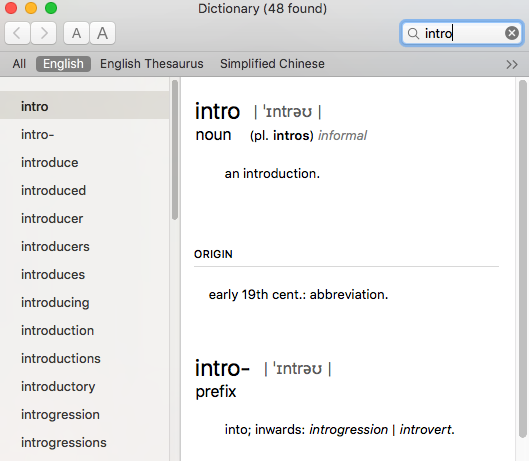
\includegraphics[scale=0.4]{img/edict-en.eps}
  \caption{E-dictionary. All candidates starting with what the user input are listed.}
  \label{fig:e-dict}
\end{figure}

A E-dictionary typically contains hundreds of thousands words. It's very expensive
to perform a complete search. Commercial software adopts complex approaches, including
caching, indexing etc to speed up this process.

Similar with e-dictionary, figure \ref{fig:word-completion} shows a popular
Internet search engine. When user input something, it provides a candidate
lists, with all items starting with what the user has entered\footnote{It's more complex than just matching the prefix. Including the spell checking and auto currection, key words extraction and recommendation etc.}. And these candidates
are shown in the order of popularity. The more people search, the
upper position it is in the list.

\begin{figure}[htbp]
  \centering
  
\includegraphics[scale=0.5]{img/adaptive-input.eps}
  \caption{A search engine. All candidates starting with what user input are listed.}
  \label{fig:word-completion}
\end{figure}

In both cases, the software provides a kind of word auto-completion mechanism.
Some editors can also help programmers to auto-complete the code.

Let's see how to implement the e-dictionary with prefix tree.
To simplify the problem, we assume the dictionary only supports English - English
information.

A dictionary stores key-value pairs, the key is English
word or phrase, the value is the meaning described in text.

We can store all the words and their meanings in a trie, but it consumes
too large space especially when there are huge amount of items. We'll use
prefix tree to realize the e-dictionary.

When user wants to look up word 'a', the dictionary does not only
return the meaning of 'a', but also provides a list of
candidates starting with 'a', including 'abandon', 'about',
'accent', 'adam', ... Of course all these words are stored in the prefix tree.

If there are too many candidates, we can limit only displaying the top 10
candidates, and allow the user to browse more.

To define this algorithm, if the string we
are looking for is empty, we expand all children sub-trees until getting $n$
candidates. Otherwise we recursively examine the children to
find one which has prefix equal to this string.

In programming environments supporting lazy evaluation. An intuitive
solution is to lazily expand all candidates, and take the first $n$ on
demand. Denote the prefix tree in form $T = (v, C)$,
below function enumerates all items starts with key $k$.

\be
findAll(T, k) = \left \{
  \begin{array}
  {r@{\quad:\quad}l}
  enum(C) & k = \phi, v = \phi \\
  \{(\phi, v)\} \cup enum(C) & k = \phi, v \neq \phi \\
  find(C, k) & k \neq \phi
  \end{array}
\right.
\ee

The first two clauses deal with the edge cases that the key is empty.
All the children sub-trees are enumerated except for those with empty values.
The last clause finds child sub-tree matches $k$.

For non-empty children sub-trees, $C = \{(k_1, T_1), (k_2, T_2), ..., (k_m, T_m)\}$,
denote the rest pairs except for the first one as $C'$.
The enumeration algorithm can be defined as below.

\be
enum(C) = \left \{
  \begin{array}
  {r@{\quad:\quad}l}
  \phi & C = \phi \\
  mapAppend(k_1, findAll(T_1, \phi)) \cup enum(C')
  \end{array}
\right.
\ee

Where $mapAppend(k, L) = \{(k + k_i, v_i)| (k_i, v_i) \in L\}$. It concatenate
the prefix $k$ in front of every key-value pair in list $L$\footnote{The concept here is to map on the first thing. In some environment, like Haskell, $mapAppend$ can be expressed as $map(first(k+), L)$ by using the arrow in category theory.}.

Function $enum$ can also be defined with concept of $concatMap$ (also called $flatMap$)\footnote{Literally, it results like first map on each element, then concatenate the result together. It's typically realized with 'build-foldr' to eliminate the intermediate list.}.

\be
enum(C) = concatMap(\lambda_{(k, T)} . mapAppend(k, findAll(T, \phi)))
\ee

Function $find(C, k)$ is defined as the following. For empty children, the
result is empty as well; Otherwise, it examines the first child sub-tree $T_1$ which
is bound to string $k_1$. If $k$ equals to $k_1$ or is a prefix of $k_1$, it calls $mapAppend$ to concatenate the prefix $k_1$ in front of the key of every child sub-tree under $T_1$; If $k_1$ is prefix
of $k$, the algorithm recursively find all children sub-trees start with $k - k_1$;
otherwise, the algorithm by-passes the first child sub-tree
and goes on finding the rest sub-trees.

\be
find(C, k) = \left \{
  \begin{array}
  {r@{\quad:\quad}l}
  \phi & C = \phi \\
  mapAppend(k_1, findAll(T_1, \phi)) & k \sqsubset k_1 \\
  mapAppend(k_1, findAll(T_1, k - k_1)) & k_1 \sqsubset k \\
  find(C', k) & otherwise
  \end{array}
\right.
\ee

Below example Haskell program implements the e-dictionary application
according to the above equations.

\lstset{language=Haskell}
\begin{lstlisting}
import Control.Arrow (first)

get n t k = take n $ findAll t k

findAll :: Eq k => PrefixTree k v -> [k] -> [([k], v)]
findAll (PrefixTree Nothing cs) [] = enum cs
findAll (PrefixTree (Just x) cs) [] = ([], x) : enum cs
findAll (PrefixTree _ cs) k = find' cs k
  where
    find' [] _ = []
    find' ((k', t') : ps) k
          | k `isPrefixOf` k'
              = map (first (k' ++)) (findAll t' [])
          | k' `isPrefixOf` k
              = map (first (k' ++)) (findAll t' $ drop (length k') k)
          | otherwise = find' ps k

enum :: Eq k => [([k], PrefixTree k v)] -> [([k], v)]
enum = concatMap (\(k, t) -> map (first (k ++)) (findAll t []))
\end{lstlisting}

In the lazy evaluation environment, the top $n$ candidates can be
gotten like $take(n, findAll(T, k))$. Appendix A has detailed definition
of $take$ function.

We can also realize this algorithm impertiavely.
The following algorithm reuses the looking up defined for prefix tree. When
finds a node bound the prefix of what we are looking for,
it expands all its children sub-trees till getting $n$ candidates.

\begin{algorithmic}[1]
\Function{Look-Up}{$T, k, n$}
  \If{$T = $ NIL}
     \State \Return $\phi$
  \EndIf
  \State $prefix \gets$ NIL
  \Repeat
    \State $match \gets$ FALSE
    \For{$\forall (k_i, T_i) \in $ \Call{Children}{$T$}}
      \If{$k$ is prefix of $k_i$}
        \State \Return \Call{Expand}{$prefix + k _i, T_i, n$}
      \EndIf
      \If{$k_i$ is prefix of $k$}
        \State $match \gets$ TRUE
        \State $k \gets k - k_i$
        \State $T \gets T_i$
        \State $prefix \gets prefix + k_i$
        \State break
      \EndIf
    \EndFor
  \Until{$\lnot match$}
  \State \Return $\phi$
\EndFunction
\end{algorithmic}

Where function \textproc{Expand}($T, prefix, n$) picks $n$ sub-trees. They
share the same prefix in $T$. It is realized as BFS (Bread-First-Search) traverse. 14.3.1 in the Chapter of search explains BFS in detail.

\begin{algorithmic}[1]
\Function{Expand}{$prefix, T, n$}
  \State $R \gets \phi$
  \State $Q \gets \{(prefix, T)\}$
  \While{$|R| < n \land Q$ is not empty}
    \State $(k, T) \gets$ \Call{Pop}{$Q$}
    \If{\Call{Data}{$T$} $\neq$ NIL}
      \State $R \gets R \cup \{(k, $ \Call{Data}{$T$} $)\}$
    \EndIf
    \For{$\forall (k_i, T_i) \in$ \Call{Children}{$T$} in sorted order}
      \State \Call{Push}{$Q, (k + k_i, T_i)$}
    \EndFor
  \EndWhile
\EndFunction
\end{algorithmic}

The following example Python program implements the e-dictionary application.
When testing if a string is prefix of another one, it uses the \texttt{find}
function provided in standard string library.

\lstset{language=Python}
\begin{lstlisting}
def lookup(t, key, n):
    if t is None:
        return []
    prefix = ""
    while True:
        match = False
        for k, tr in t.subtrees.items():
            if string.find(k, key) == 0: # key is prefix of k
                return expand(prefix + k, tr, n)
            if string.find(key, k) ==0:
                match = True
                key = key[len(k):]
                t = tr
                prefix += k
                break
        if not match:
            break
    return []

def expand(prefix, t, n):
    res = []
    q = [(prefix, t)]
    while len(res)<n and q:
        (s, p) = q.pop(0)
        if p.value is not None:
            res.append((s, p.value))
        for k, tr in sorted(p.subtrees.items()):
            q.append((s + k, tr))
    return res
\end{lstlisting}


%=====================================
% T9
%=====================================

\subsection{T9 input method}
\index{T9}
\index{Textonym input method}

When people edit text in the mobile phone, the experience is quite different.
This is because the so called ITU-T key pad has much fewer
keys than PC as shown in figure \ref{fig:itut-keypad}.

\begin{figure}[htbp]
  \centering
  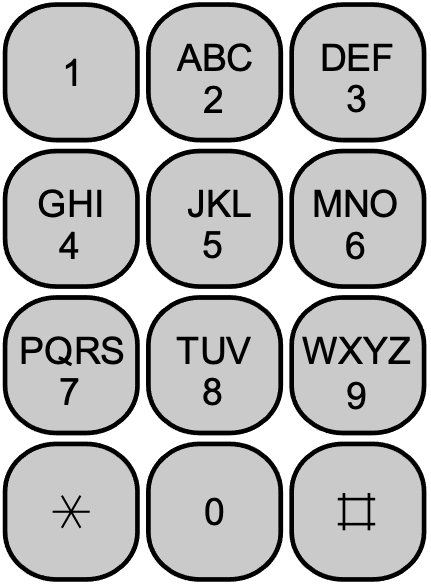
\includegraphics[scale=0.4]{img/itu-t.eps}
  \caption{The ITU-T keypad for mobile phone.}
  \label{fig:itut-keypad}
\end{figure}

There are typical two methods to input word or phrases with ITU-T key pad.
If user wants to enter a word `home' for example, he can press the keys
in below sequence.

\begin{itemize}
\item Press key '4' twice to enter the letter 'h';
\item Press key '6' three times to enter the letter 'o';
\item Press key '6' to enter the letter 'm';
\item Press key '3' twice to enter the letter 'e';
\end{itemize}

Another much quicker way is to just press the following keys.

\begin{itemize}
\item Press key '4', '6', '6', '3', word `home' appears on top of the candidate list;
\item Press key '*' to change a candidate word, so word `good' appears;
\item Press key '*' again to change another candidate word, next word `gone' appears;
\item ...
\end{itemize}

Compare the two methods, the second one is much easier for the user.
The only overhead is the need to store a dictionary of candidate words.

The second method is known as `T9' input method, or predictive input method
\cite{wiki-t9}, \cite {wiki-predictive-text}. The abbreviation 'T9' stands
for 'textonym'. It start with 'T' with 9 characters. T9 input can also be
realized with prefix tree.

In order to provide candidate words, a dictionary must be prepared
in advance. Prefix tree can be used to store the dictionary. The
commercial T9 implementations typically use multiple layers indexed dictionary in
both file system and cache. The realization shown here is for illustration
purpose only.

Firstly, we need define the T9 mapping, which maps from digit to candidate
characters.

\be
\begin{array}{ll}
M_{T9} = \{ & 2 \rightarrow abc, 3 \rightarrow def, 4 \rightarrow ghi, \\
           & 5 \rightarrow jkl, 6 \rightarrow mno, 7 \rightarrow pqrs, \\
           & 8 \rightarrow tuv, 9 \rightarrow wxyz \}
\end{array}
\ee

With this mapping, $M_{T9}[i]$ returns the corresponding characters for digit $i$. We can also define the reversed mapping from a character back to digit.

\be
M^{-1}_{T9} = concat(\{\{c \rightarrow d | c \in S\} | (d \rightarrow S) \in M_{T9}\})
\ee

Given a sequence of characters, we can convert it to a sequence of digits by looking up $M^{-1}_{T9}$.

\be
digits(S) = \{ M^{-1}_{T9}[c]| c \in S \}
\ee

When input digits $D = d_1d_2...d_n$, we define the T9 lookup algorithm as below.

\be
findT9(T, D) = \left \{
  \begin{array}
  {r@{\quad:\quad}l}
  \{ \phi \} & D = \phi \\
  concatMap(find, prefixes(T)) & otherwise
  \end{array}
\right.
\ee

Where $T$ is the prefix tree built from a set of words and phrases. It's kind of a dictionary we'll look up. If the input
$D$ is empty, the result is an empty string. Otherwise, it looks up the sub-trees that match the input, and concat the result together.

To enumerate the matched sub-trees, we examine all the children sub-trees $C_T$,
for every pair $(k_i, T_i)$. We first convert string $k_i$ to digit sequence $d_i$,
then compare $d_i$ and $D$. If either one is the prefix of the other, then this pair
is selected as a candidate for further search.

\be
prefixes(T) = \{(k_i, T_i) | (k_i, T_i) \in C_T, d_i = digits(k_i), d_i \sqsubset D \lor D \sqsubset d_i \}
\ee


Function $find$ takes a passed in prefix $S$, and a sub-tree $T'$ to look up further. As $S$ is prefix of $D$, it removes it from $D$ to get a new input to $D' = D - S$ to search, then later insert $S$ back in front of every recursive search result.

\be
find(S, T') = \{ take(n, S + s_i) | s_i \in findT9(T', D - S) \}
\ee

Where $n = |D|$ is the length of the input digits. Function $take(n, L)$ takes the first $n$ elements from the list $L$. If the length of the list is less then $n$, or the elements are taken.

The following Haskell example program implements the T9 look up algorithm with prefix tree.

\lstset{language=Haskell}
\begin{lstlisting}
import qualified Data.Map as Map

mapT9 = Map.fromList [('1', ",."), ('2', "abc"), ('3', "def"), ('4', "ghi"),
                      ('5', "jkl"), ('6', "mno"), ('7', "pqrs"), ('8', "tuv"),
                      ('9', "wxyz")]

rmapT9 = Map.fromList $ concatMap (\(d, s) -> [(c, d) | c <- s]) $ Map.toList mapT9

digits = map (\c -> Map.findWithDefault '#' c rmapT9)

findT9 :: PrefixTree Char v -> String -> [String]
findT9 t [] = [""]
findT9 t k = concatMap find prefixes
  where
    n = length k
    find (s, t') = map (take n . (s++)) $ findT9 t' (k `diff` s)
    diff x y = drop (length y) x
    prefixes = [(s, t') | (s, t') <- children t, let ds = digits s in
                          ds `isPrefixOf` k || k `isPrefixOf` ds]
\end{lstlisting}

To realize this algorithm imperatively, we can perform BFS search with a queue $Q$.
The queue stores tuples $(prefix, D, T)$. Every tuple records the possible
prefix string we've searched so far; the rest of the digits to be searched;
and the sub-tree we are going to search. The queue is initialized with the
empty prefix, the whole digit sequence, and the prefix tree root. The algorithm
keeps picking the tuple from the queue until it's empty. For every tuple
popped from the queue, we extract the tree from the tuple, then examine the
children sub-trees of it. for each sub-tree $T_i$, we convert the corresponding
prefix string $k_i$ to digits $D'$ by looking up the reversed T9 map. If the
$D$ is prefix of $D'$, it's a valid candidate. We concatenate $k_i$ after
the prefix in the tuple, and record this string in the result. If $D'$ is
prefix of $D$, we need furthur search this sub-tree. To do this, we
create a new tuple consist of the new prefix ends with $k_i$, the rest of
the digits $D-D'$, and the sub-tree. Then push this tuple back to the queue.

\begin{algorithmic}[1]
\Function{Look-Up-T9}{$T, D$}
  \State $R \gets \phi$
  \If{$T =$ NIL or $D = \phi$}
    \State \Return $R$
  \EndIf
  \State $n \gets |D|$
  \State $Q \gets \{(\phi, D, T)\}$
  \While{$Q \neq \phi$}
    \State $(prefix, D, T) \gets$ \Call{Pop}{$Q$}
    \For{$\forall (k_i, T_i) \in $ \Call{Children}{$T$}}
      \State $D' \gets$ \Call{Digits}{$k_i$}
      \If{$D' \sqsubset D$} \Comment{$D'$ is prefix of $D$}
        \State $R \gets R \cup \{$ \textproc{Take} $(n, prefix + k_i) \}$ \Comment{limit the length to $n$}
      \ElsIf{$D \sqsubset D'$}
        \State \textproc{Push}($Q, (prefix + k_i, D - D', T_i)$)
      \EndIf
    \EndFor
  \EndWhile
  \State \Return $R$
\EndFunction
\end{algorithmic}

Function \textproc{Digits}($S$) converts string $S$ to sequence of digits.

\begin{algorithmic}[1]
\Function{Digits}{$S$}
  \State $D \gets \phi$
  \For{each $c \in S$}
    \State $D \gets D \cup \{M^{-1}_{T9}[c]\}$
  \EndFor
  \State \Return $D$
\EndFunction
\end{algorithmic}

The following example Python program implements the T9 input method with prefix tree.

\lstset{language=Python}
\begin{lstlisting}
T9MAP={'2':"abc", '3':"def", '4':"ghi", '5':"jkl", \
       '6':"mno", '7':"pqrs", '8':"tuv", '9':"wxyz"}

T9RMAP = dict([(c, d) for d, cs in T9MAP.items() for c in cs])

def digits(w):
    return ''.join([T9RMAP[c] for c in w])

def lookup_t9(t, key):
    if t is None or key == "":
        return []
    res = []
    n = len(key)
    q = [("", key, t)]
    while q:
        prefix, key, t = q.pop(0)
        for k, tr in t.subtrees.items():
            ds = digits(k)
            if string.find(ds, key) == 0: # key is prefix of ds
                res.append((prefix + k)[:n])
            elif string.find(key, ds) == 0: # ds is prefix of key
                q.append((prefix + k, key[len(k):], tr))
    return res
\end{lstlisting}


\begin{Exercise}
\begin{itemize}
\item Realize the e-dictionary and T9 lookup with trie.
\item For the alphabetic prefix tree look up algorithms that return multiple results, how to ensure the result is in lexicographic order? What is the performance?
\item How to realize the e-dictionary and T9 look up without lazy evaluation?
\end{itemize}
\end{Exercise}

% ================================================================
%                 Short summary
% ================================================================
\section{Summary}

In this chapter, we start from the integer based trie and prefix tree. The
map data structure based on integer tree plays the important role
in Compiler implementation. Alphabetic trie and prefix tree are
natural extensions. They can manipulate text information.
We demonstrate how to realize the predictive e-dictionary
and T9 input method with prefix tree, although these examples
are different from the commercial implementations.
Other data structure, suffix tree, has close
relationship with trie and prefix tree. Suffix tree is introduced
in Appendix D.

\begin{thebibliography}{99}

\bibitem{CLRS}
Thomas H. Cormen, Charles E. Leiserson, Ronald L. Rivest and Clifford Stein.
``Introduction to Algorithms, Second Edition''. Problem 12-1. ISBN:0262032937. The MIT Press. 2001

\bibitem{okasaki-int-map}
Chris Okasaki and Andrew Gill. ``Fast Mergeable Integer
Maps''. Workshop on ML, September 1998, pages 77-86, \url{http://www.cse.ogi.edu/~andy/pub/finite.htm}

\bibitem{patricia-morrison}
D.R. Morrison, ``PATRICIA -- Practical Algorithm To Retrieve  Information Coded In Alphanumeric", Journal of the ACM, 15(4), October 1968, pages 514-534.

\bibitem{wiki-suffix-tree}
Suffix Tree, Wikipedia. \url{http://en.wikipedia.org/wiki/Suffix_tree}

\bibitem{wiki-trie}
Trie, Wikipedia. \url{http://en.wikipedia.org/wiki/Trie}

\bibitem{wiki-t9}
T9 (predictive text), Wikipedia. \url{http://en.wikipedia.org/wiki/T9_(predictive_text)}

\bibitem{wiki-predictive-text}
Predictive text,
Wikipedia. \url{http://en.wikipedia.org/wiki/Predictive_text}

\end{thebibliography}

\ifx\wholebook\relax\else
\end{document}
\fi
